\documentclass[tikz, border=10pt]{standalone}
\usepackage{tikz}
\usepackage[utf8]{inputenc}
\usepackage[T1]{fontenc}
\usepackage{amsmath}
\usetikzlibrary{arrows.meta, fit, backgrounds, calc}

\colorlet{col1}{green!55!black}
\colorlet{col2}{blue!60!black}
\colorlet{col3}{orange!65!black}
\colorlet{col4}{violet!60!black}

\tikzset{
  nd/.style={
    draw=gray!55, fill=white, rounded corners=5pt,
    font=\footnotesize, text centered, align=center,
    minimum height=1.05cm, inner sep=4pt, thick
  },
  cnd/.style={nd, draw=#1!85, fill=#1!11},
  ph/.style={minimum width=0pt, minimum height=0pt,
             inner sep=0pt, outer sep=0pt, draw=none, fill=none},
  sbox/.style={draw=#1, line width=2pt, rounded corners=8pt,
               fill=#1!6, inner sep=10pt},
  ar/.style={-{Stealth[length=2.6mm, width=1.9mm]}, thick, #1},
  sar/.style={-{Stealth[length=2.9mm, width=2.3mm]}, line width=1.4pt, gray!55},
  snum/.style={circle, fill=#1, draw=#1, text=white, font=\bfseries\small,
               minimum size=6.5mm, inner sep=0pt},
  stit/.style={font=\bfseries\scriptsize, text=#1},
}

%%  LEFT col x in [-0.05, 7.25]   RIGHT col x in [8.75, 16.05]
\def\XLL{-0.05}  \def\XLR{7.25}
\def\XRL{8.75}   \def\XRR{16.05}
\def\Ytop{1.1}   %% headroom above top content row for title + circle

\begin{document}
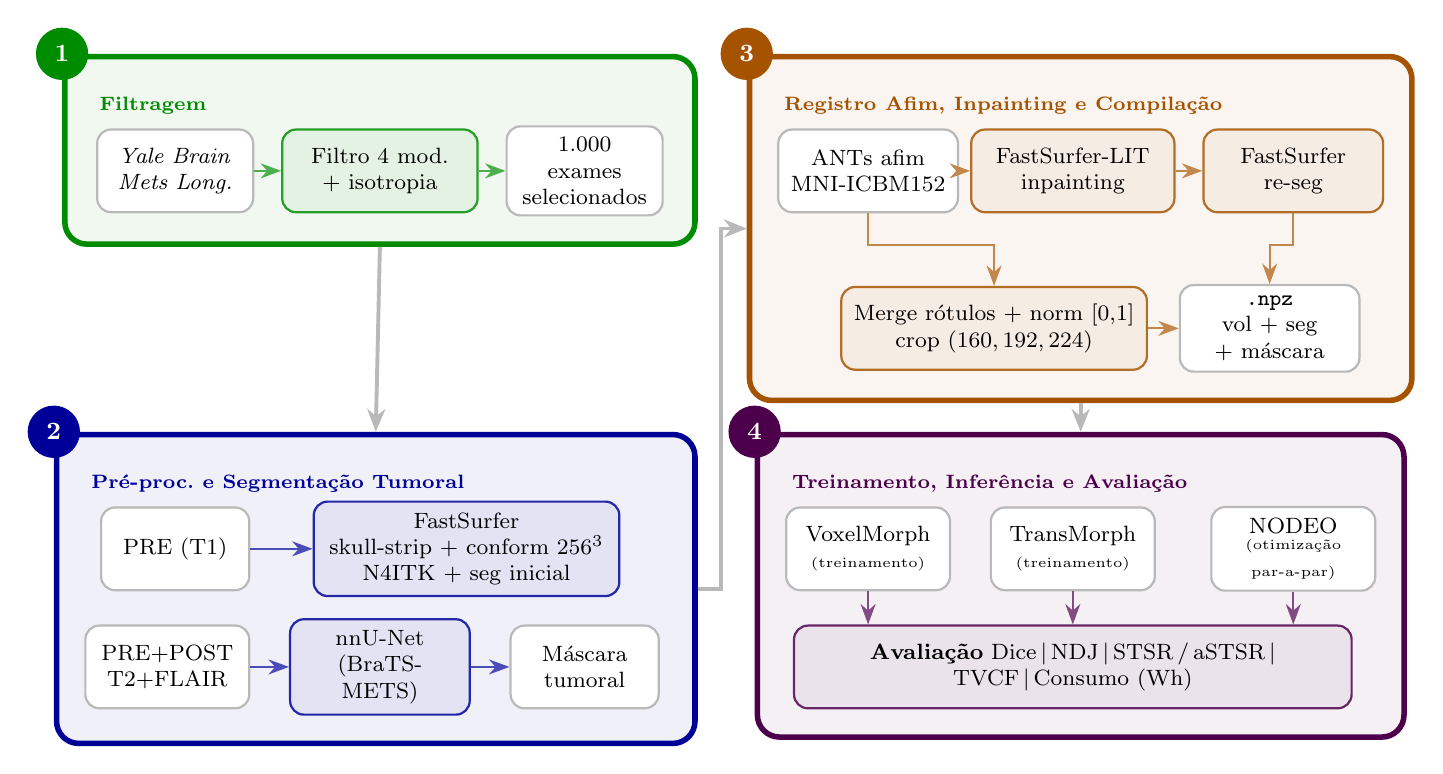
\begin{tikzpicture}

%% ============================================================
%% LEFT COLUMN
%% ============================================================

%% --- 1. FILTRAGEM  (left, TOP) ---  content row at y = 0
\node[nd, text width=1.7cm] (n1a) at (1.0, 0)
  {\textit{Yale Brain}\\\textit{Mets Long.}};
\node[cnd=col1, text width=2.2cm] (n1b) at (3.6, 0)
  {Filtro 4 mod.\\+ isotropia};
\node[nd, text width=1.7cm] (n1c) at (6.2, 0)
  {1.000\\exames\\selecionados};

\draw[ar=col1!70] (n1a) -- (n1b);
\draw[ar=col1!70] (n1b) -- (n1c);

\node[ph] (s1L) at (\XLL, \Ytop)  {};
\node[ph] (s1R) at (\XLR, \Ytop)  {};
\begin{scope}[on background layer]
  \node[sbox=col1, fit=(n1a)(n1b)(n1c)(s1L)(s1R)] (box1) {};
\end{scope}
\node[snum=col1] at (box1.north west) {\bf 1};
\node[stit=col1, anchor=north west]
  at ([xshift=10pt, yshift=-12pt] box1.north west) {Filtragem};


%% --- 2. PRE-PROC. E SEGMENTACAO  (left, BOTTOM) ---  rows at y = -4.8 / -6.3
%%       aligned with box 4 -> clean 2x2 grid, reaches image bottom
\node[nd, text width=1.6cm] (n2a) at (1.0, -4.8) {PRE (T1)};
\node[cnd=col2, text width=3.6cm] (n2b) at (4.7, -4.8)
  {FastSurfer\\skull-strip + conform $256^3$\\N4ITK + seg inicial};

\node[nd, text width=1.8cm] (n2c) at (0.9, -6.3) {PRE+POST\\T2+FLAIR};
\node[cnd=col2, text width=2.0cm] (n2d) at (3.6, -6.3) {nnU-Net\\(BraTS-METS)};
\node[nd, text width=1.6cm]  (n2e) at (6.2, -6.3) {M\'{a}scara\\tumoral};

\draw[ar=col2!70] (n2a) -- (n2b);
\draw[ar=col2!70] (n2c) -- (n2d);
\draw[ar=col2!70] (n2d) -- (n2e);

\node[ph] (s2L) at (\XLL, {-4.8+\Ytop}) {};
\node[ph] (s2R) at (\XLR, {-4.8+\Ytop}) {};
\begin{scope}[on background layer]
  \node[sbox=col2, fit=(n2a)(n2b)(n2c)(n2d)(n2e)(s2L)(s2R)] (box2) {};
\end{scope}
\node[snum=col2] at (box2.north west) {\bf 2};
\node[stit=col2, anchor=north west]
  at ([xshift=10pt, yshift=-12pt] box2.north west)
  {Pr\'{e}-proc.\ e Segmenta\c{c}\~{a}o Tumoral};

\draw[sar] (box1.south) -- (box2.north);


%% ============================================================
%% RIGHT COLUMN
%% ============================================================

%% --- 3. REGISTRO AFIM, INPAINTING E COMPILACAO  (right, TOP) ---  rows at y = 0 / -1.7
\node[nd, text width=2.0cm]  (n3a) at (9.8,  0) {ANTs afim\\MNI-ICBM152};
\node[cnd=col3, text width=2.3cm] (n3b) at (12.4, 0) {FastSurfer-LIT\\inpainting};
\node[cnd=col3, text width=2.0cm] (n3c) at (15.2, 0) {FastSurfer\\re-seg};

\draw[ar=col3!70] (n3a) -- (n3b);
\draw[ar=col3!70] (n3b) -- (n3c);

\node[cnd=col3, text width=3.6cm] (n3d) at (11.4, -2.0)
  {Merge r\'{o}tulos + norm $[0,\!1]$\\crop $(160,192,224)$};
\node[nd, text width=2.0cm]  (n3e) at (14.9, -2.0)
  {\texttt{.npz}\\vol + seg\\+ m\'{a}scara};

%% ANTs afim -> Merge (down-left)
\draw[ar=col3!70] (n3a.south) -- ++(0,-0.40) -| (n3d.north);
%% FastSurfer re-seg -> .npz (down)
\draw[ar=col3!70] (n3c.south) -- ++(0,-0.40) -| (n3e.north);
%% Merge -> .npz (horizontal)
\draw[ar=col3!70] (n3d) -- (n3e);

\node[ph] (s3L) at (\XRL, \Ytop)  {};
\node[ph] (s3R) at (\XRR, \Ytop)  {};
\begin{scope}[on background layer]
  \node[sbox=col3, fit=(n3a)(n3b)(n3c)(n3d)(n3e)(s3L)(s3R)] (box3) {};
\end{scope}
\node[snum=col3] at (box3.north west) {\bf 3};
\node[stit=col3, anchor=north west]
  at ([xshift=10pt, yshift=-12pt] box3.north west)
  {Registro Afim, Inpainting e Compila\c{c}\~{a}o};


%% --- 4. TREINAMENTO, INFERENCIA E AVALIACAO  (right, BOTTOM) ---  rows at y = -4.5 / -6.0
\node[nd, text width=1.8cm] (n4a) at (9.8,  -4.8) {VoxelMorph\\{\tiny (treinamento)}};
\node[nd, text width=1.8cm] (n4b) at (12.4, -4.8) {TransMorph\\{\tiny (treinamento)}};
\node[nd, text width=1.8cm] (n4c) at (15.2, -4.8)
  {NODEO\\{\tiny (otimiza\c{c}\~{a}o\\par-a-par)}};

\node[cnd=col4, text width=6.8cm] (n4d) at (12.4, -6.3)
  {\textbf{Avalia\c{c}\~{a}o}
   Dice\,$|$\,NDJ\,$|$\,STSR\,/\,aSTSR\,$|$\\
   TVCF\,$|$\,Consumo (Wh)};

\draw[ar=col4!70] (n4a.south) -- (n4d.north -| n4a.south);
\draw[ar=col4!70] (n4b.south) -- (n4d.north -| n4b.south);
\draw[ar=col4!70] (n4c.south) -- (n4d.north -| n4c.south);

\node[ph] (s4L) at (\XRL, {-4.8+\Ytop}) {};
\node[ph] (s4R) at (\XRR, {-4.8+\Ytop}) {};
\begin{scope}[on background layer]
  \node[sbox=col4, fit=(n4a)(n4b)(n4c)(n4d)(s4L)(s4R)] (box4) {};
\end{scope}
\node[snum=col4] at (box4.north west) {\bf 4};
\node[stit=col4, anchor=north west]
  at ([xshift=10pt, yshift=-12pt] box4.north west)
  {Treinamento, Infer\^{e}ncia e Avalia\c{c}\~{a}o};

\draw[sar] (box3.south) -- (box4.north);


%% Cross-column: box2 (bottom-left) -> box3 (top-right)
%% short horizontal stub out of box2.east, then up into box3.west
\draw[sar] (box2.east) -- ++(0.3,0) |- (box3.west);

\end{tikzpicture}
\end{document}
